\newcommand{\plotfraction}{0.85}
Historically, dxex is based on PythonPDEVS~\cite{PythonPDEVS}.
Python is a good language for prototypes, but performance has proven insufficient to compete with other simulation kernels~\cite{MasterThesis}.
Dxex is a C++11-based implementation of PythonPDEVS, but implements only a subset of PythonPDEVS, while making some of its own additions.
So while the feature set is not too comparable, the architectural design, core simulation algorithm, and optimizations, are highly similar.

We will not make a detailed comparison with PythonPDEVS here, but only mention some supported features.
Dxex supports, similarly to PythonPDEVS, the following features: direct connection~\cite{SymbolicFlattening}, \textsf{Dynamic Structure DEVS}~\cite{DSDEVS}, termination conditions, and a modular tracing and scheduling framework~\cite{PythonPDEVS}.
But whereas PythonPDEVS only supports optimistic synchronization, dxex support multiple synchronization protocols (though only in parallel).
This is in line with the design principle of PythonPDEVS: allow users to pass performance hints to the simulation kernel.
In our case, a user can pass the simulation kernel the synchronization protocol to use for this model, or even switch the synchronization protocol during runtime.
Our implementation in C++11 also allows for optimizations which were plainly impossible in an interpreted language. Dxex will use new optimizations from the C++14 standard when possible.

Since there is no universal \textsf{DEVS} model standard, dxex models are incompatible with PythonPDEVS and vice versa.
This is due to dxex models being grafted on C++11, whereas PythonPDEVS models are grafted on Python.

In the remainder of this section, we will elaborate on our prominent new feature: the efficient implementation of multiple synchronization protocols within the same simulation tool, which are offered transparently to the model.

\subsection{Synchronization protocols}
We previously explained the existence of different synchronization protocols, each optimized for a specific kind of model.
As no single synchronization protocol is ideal for all models, a general purpose simulation tool should support multiple protocols.
Currently, most parallel simulation tools choose only a single synchronization protocol due to the inherent differences between protocols.
An uninformed choice on which one to implement is insufficient, as performance will likely be bad.
We argue that a real general purpose simulation tool should support sequential, conservative, and optimistic synchronization, as is the case for dxex.

These different protocols relate to three different model characteristics.
Conservative synchronization for when high lookahead exists between different nodes, and barely any blocking is necessary.
Optimistic synchronization for when lookahead is unpredictable, or there are rare (almost) instantaneous events.
Finally, sequential simulation is still required for models where parallelism is bad, where all protocols actually slow down simulation.

\subsubsection{Sequential}
Our sequential simulation algorithm is very similar to the one found in PythonPDEVS, including many optimizations.
Minor modifications were made, though, such that it can be overloaded by different synchronization protocol implementations.
This way, the \textsf{DEVS} simulation algorithm is implemented once, but parts can be overridden as needed.
In theory, more synchronization protocols (\textit{e.g.}, other algorithms for conservative synchronization) can be added without altering our design.

An overview of dxex's design is given in Figure~\ref{fig:class_diagram}.
It shows that there is a simulation \texttt{Core}, which simulates the \texttt{AtomicModel}s connected to it.
The superclass \texttt{Core} is merely the sequential simulation core, but can be used as-is.
Subclasses define specific variants, such as \texttt{ConservativeCore} (conservative synchronization), \texttt{OptimisticCore} (optimistic synchronization), and \texttt{DynamicCore} (\textsf{Dynamic Structure DEVS}).

\begin{figure}
    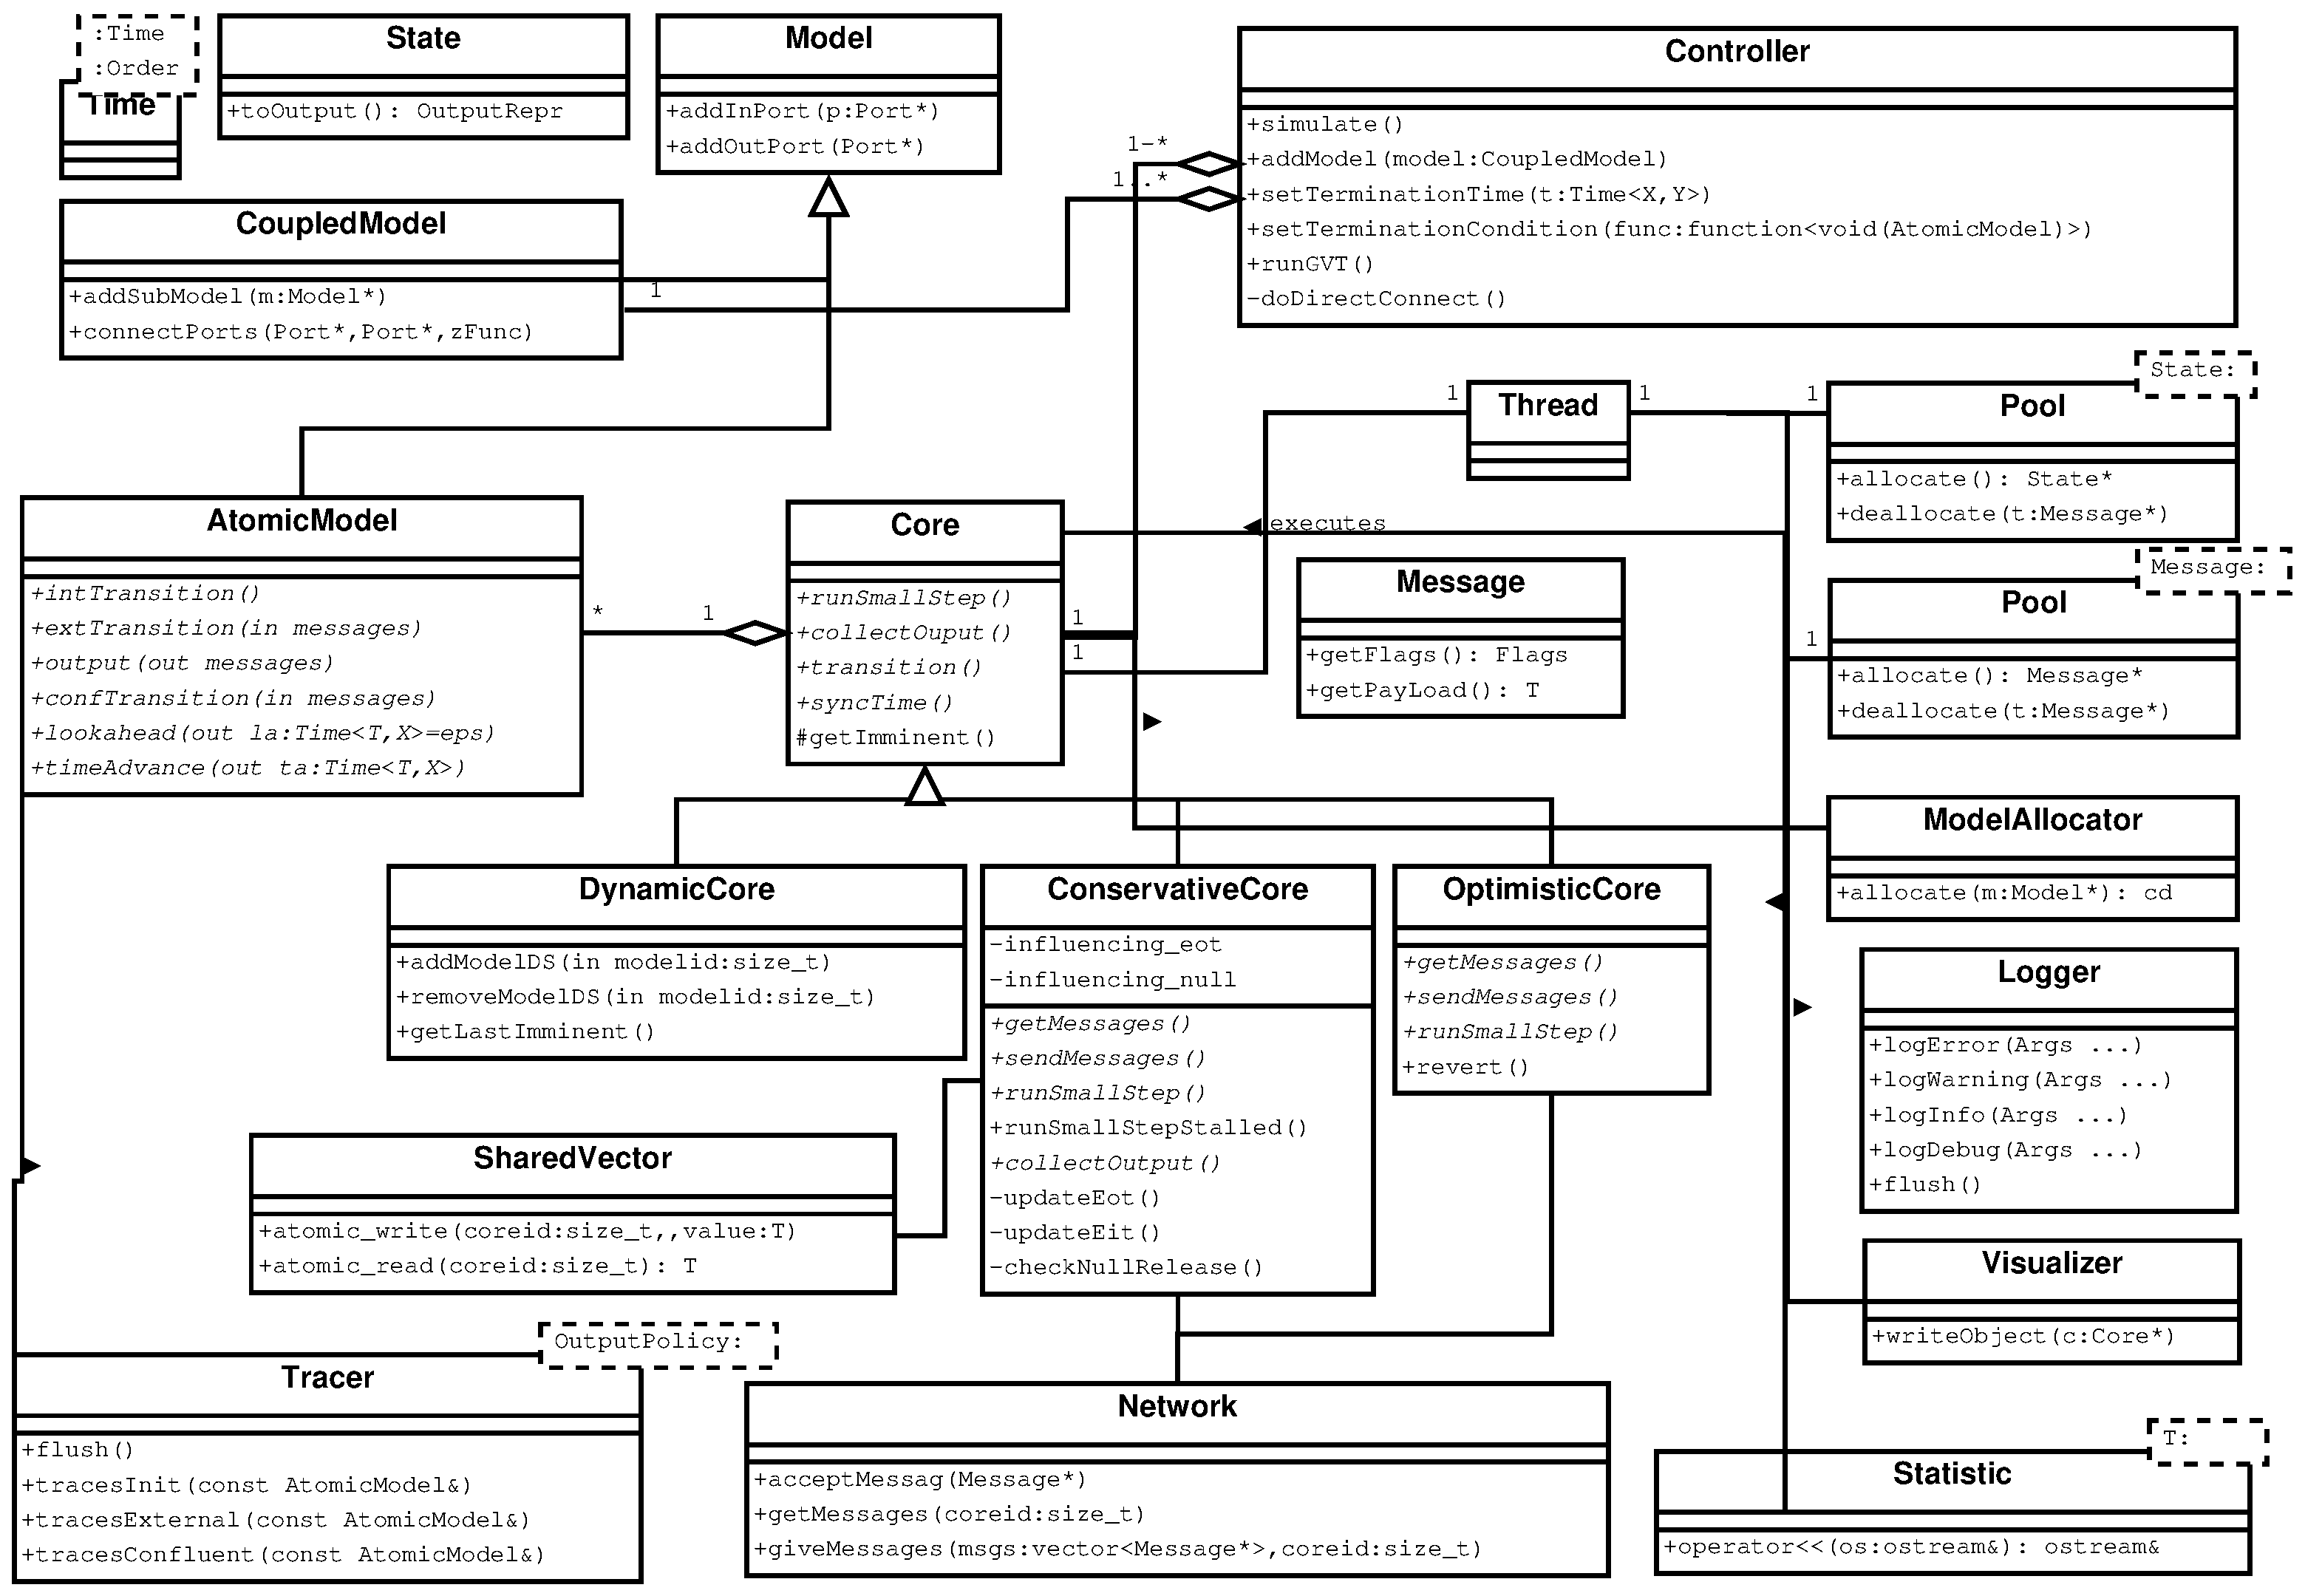
\includegraphics[width=\columnwidth]{fig/cores_class_diagram.eps}
	\caption{Dxex design.}
	\label{fig:class_diagram}
\end{figure}

\subsubsection{Conservative}
For conservative synchronization, each node must determine the nodes it is influenced by.
Each model needs to provide a lookahead function, which determines the lookahead depending on the current simulation state.
Within the returned time interval, the model promises not to raise an event.
A node aggregates this information to compute its earliest output time (EOT).
This value is written out in shared memory, where it can be read out by all other nodes.

Reading and writing to shared memory is done through the use of the new C++11 synchronization primitives.
Whereas this was also possible in previous versions of the C++ standard, by falling back to non-portable C functions, it was not a part of the C++ language standard.
C++11 further allows us to make the implementation portable, as well as more efficient: the compiler might know of optimizations specific to atomic variables or constant expressions which are heavily used in dxex.

\subsubsection{Optimistic}
For optimistic synchronization, each node must be able to roll back to a previous point in time.
This is often implemented through the use of state saving.
This needs to be done carefully in order to avoid unnecessary copies, and minimize the overhead.
We use the default: explicitly save each and every intermediate state.
Mattern's algorithm~\cite{mattern} is used to determine the GVT, as it runs asynchronously and uses only $2n$ synchronization messages.
Once the GVT is found, all nodes are informed of the new value, after which fossil collection is performed, and irreversible actions are committed.

The main problem we encountered in our implementation is the aggressive use of memory.
Frequent memory allocation and deallocation caused significant overheads, certainly when multiple threads do so concurrently.
This made us switch to the use of thread-local (using \texttt{tcmalloc}) memory pools.
Again, we made use of specific new features of C++11, that were not available in Python, or even previous versions of the C++ language standard.

\subsection{Synchronization Protocol Transparency}
We define synchronization protocol transparency as having a single model, which always can be executed on each supported synchronization kernel, without any modifications.
User should thus only provide one model, implemented in C++11, which can be either using sequential execution, using conservative synchronization, or using optimistic synchronization.
Switching between simulation kernels is as simple as altering the simulation termination time.
The exception is conservative synchronization, where a lookahead function is required, which is not used in other synchronization kernels.
Two options are possible: either a lookahead function must always be provided, even when it is not required and possibly not used, or we use a default lookahead function if none is defined.

Always defining a lookahead function might seem redundant, especially if users will never use conservative synchronization.
Especially since defining the lookahead is often non-trivial and dependent on intricate model details.
The more attractive option is for the simulation tool to provide a default lookahead function, such that simulation can run anyway, but likely not at peak performance.
Depending on the model, simulation performance might still be faster than sequential simulation. 

Defining a lookahead function is therefore recommended in combination with conservative synchronization, but is not a necessity, as a default $epsilon$ (\textit{i.e.}, the smallest representable timestep) is used otherwise.

\subsection{Increasing Parallelism}
The simulation kernels have a non trivial overhead compared to a sequential kernel. In this section we will try to isolate this overhead.

Profiling indicates that there are in the most trivial of models only 2 causes for computational load outside of the actual simulation : memory management and random number generation. By reducing the cost of both we will isolate the synchronization overhead. We use the Queue benchmark since it is highly parallel and its computational load in transitioning is only determined by random number generation and event/state allocation.

\subsubsection{Memory Management}
\label{sec:4-subsec:overhead-pgraph:memory}
\begin{figure}
    \center

    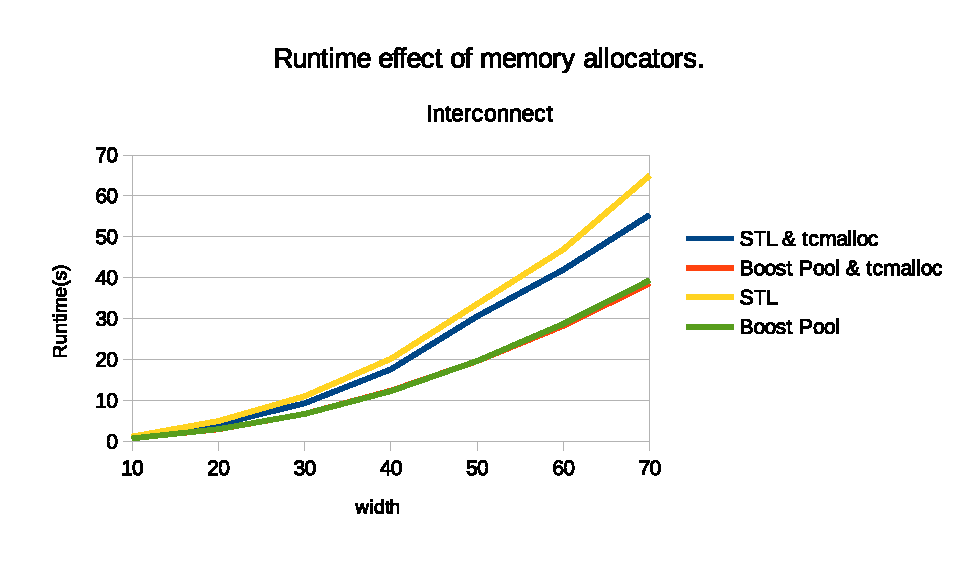
\includegraphics[width=\modelfraction\columnwidth]{fig/memory_allocators.eps}
    \caption{Effect of memory allocators on sequential runtime.}
    \label{fig:memallocators}

    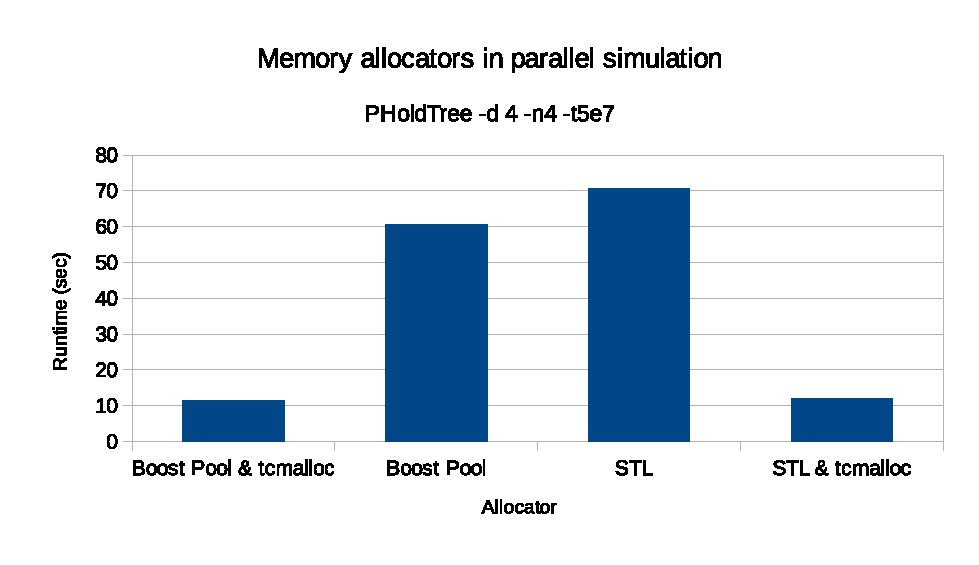
\includegraphics[width=\modelfraction\columnwidth]{fig/memory_allocators_parallel.eps}
    \caption{Effect of memory allocators on parallel runtime.}
    \label{fig:memallocators_parallel}
\end{figure}
In dxex a model author is given access to automatic memory management for events and states. A model written for a sequential simulation will run correctly in a conservative or optimistic simulation without altering (from the point of view of the model author) the (de)allocation semantics of events or states. \\
In sequential and conservative simulation the kernel gives the guarantee that no state will be copied. Dxex's simulation control hides the implementation details of this management, a model author can focus on the actual semantics of the model.
The kernels use memory allocators backed by a thread-aware pooling library to reduce the performance impact of memory management as much as possible.
In a sequential simulation kernel no allocated event will persist beyond a single time advance, allowing the use of an arena-style allocator. Conservative and optimistic simulation need to use generic pool allocators since events are shared across kernels and thus have a different lifetime. \\
An important observation to make is that intra-kernel events can be pooled more aggressively, whereas inter-kernel events need a GVT algorithm to determine when safe deallocation can occur, even in conservative synchronization. A simulation with high inter kernel events will suffer a performance hit, whereas the impact of high intra kernel events can be optimized using arena allocators.\\
The allocation interfaces are instrumented in dxex to trace memory usage in a simulation and can serve as a basic memory leak detector. Shielding the user from (de)allocation complexity comes at a cost in performance, as the comparison with adevs in simulations with a high event frequency \ref{fig:Interconnect_benchmark} of events shows.\\
\\
Dxex uses Boost Pool\cite{boostpool} allocators in parallel simulation kernels and arena-style allocators for sequential simulation.
The latter can be faster, but at the cost of extra configuration. The allocators are supplemented by the library tcmalloc \cite{tcmalloc}. In Figure \ref{fig:memallocators} the Interconnect model is benchmarked under the different combinations of allocation strategies. \\
Interconnect is a perfect test case since it generates each round a set of events quadratic in size to the number of atomic models in the simulation. With each event dynamically allocated, this makes it the perfect stress test for any allocation strategy. Both tcmalloc and Boost pools result in an advantage, but not necessarily combined. \\
We next investigate the effect of both strategies in an optimistic simulation. We have already demonstrated that conservative simulation differs little in memory usage from sequential, so we only benchmark the optimistic kernel. From the results it is clear that optimistic simulation benefits greatly from the use of tcmalloc, regardless of the allocator. Nonetheless the pool allocator still reduces the allocation overhead. \\
Both the pools and tcmalloc will try to keep memory allocated to them by the OS, this gives a somewhat misleading view in statistics collected from the OS. The dxex kernels themselves and the pool interfaces allow the user to instrument event allocation and deallocation exactly which can be useful in measuring how efficient GVT-triggered deallocation is in practice.\\
In conclusion both techniques are required to reduce the overhead of memory allocations in dxex, and on by default.

\subsubsection{Random Number Generators}
A non trivial amount of time in a simulation spent waiting for a random number generator (rng) can mask synchronization overhead. Several of our benchmarks use random number generators to test the effect of uncertainty in a simulation, either by random time advances or random destinations for events. \\
In a parallel simulation we also need to guarantee isolation between the random calls to avoid excessive synchronization on the rng object itself.
Dxex uses the Tina random number generator collection (trng) \cite{PhysRevE.75.066701} as an alternative random number generator as it is designed with performance and multithreading usage in mind.
We also wrote a new version of our models that stores the rng object in the state instead of calling a shared thread local object to isolate the synchronization overhead.\\
From Figure \ref{fig:Queuerngspeedup} we see that storing the rng in the state is a very expensive operation for the default STL random number generator. The size of the rng object in the state triggers memory overhead but it is interesting to see that adevs' conservative is also sensitive to this effect even though in theory in conservative synchronization no state copying/saving is required.
Dxex's conservative kernel is insensitive to storing the rng object in the atomic model state, since no copying/state saving occurs in dxex conservative simulation. \\
Replacing the STL rng with the threading optimized trng we are more accurately able to isolate synchronization overhead. Figure \ref{fig:Queuerngspeedup} shows that both dxex and adevs in sequential simulation gain a factor ~3 speedup by using the faster random number generator. The parallel kernels have a smaller speedup with adevs' conservative and dxex optimistic achieving an almost identical factor. Dxex conservative is almost insensitive to the changing of the rng.
Dxex optimistic and adevs conservative in the default configuration spend relatively more time waiting for random numbers than dxex conservative, demonstrated by the speedup gained when random number generation is accelerated.
The actual synchronization overhead in all parallel kernels still dominates the cost of random number generation which is seen from the speedup difference between parallel and sequential.\\
\begin{figure}
    \center

    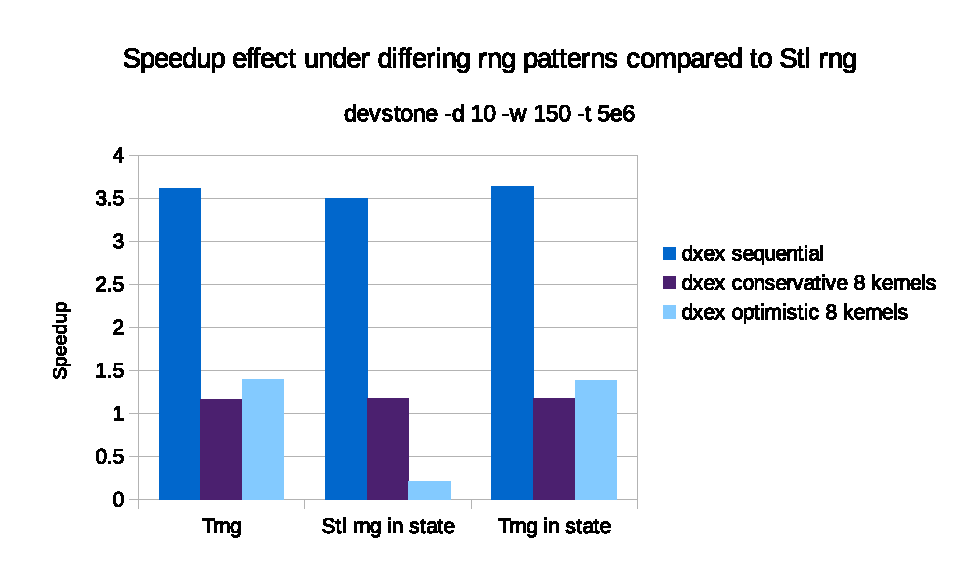
\includegraphics[width=\modelfraction\columnwidth]{fig/rngspeedupeffectdevstone.eps}
    \caption{Speedup with different rng usage patterns in Queue model}
    \label{fig:Queuerngspeedup}

\end{figure}
